\documentclass[10pt,mathserif]{beamer}

\usepackage{graphicx,amsmath,amssymb}
\usepackage{subcaption, natbib, hyperref}
\hypersetup{
    colorlinks=true,
    linkcolor=blue,
    filecolor=magenta,
    urlcolor=cyan,
}

% ------------------------------------------------------------------------
% Packages
% ------------------------------------------------------------------------
\usepackage{amsmath}

% ------------------------------------------------------------------------
% Macros
% ------------------------------------------------------------------------
%~~~~~~~~~~~~~~~
% List shorthand
%~~~~~~~~~~~~~~~
\newcommand{\BIT}{\begin{itemize}}
\newcommand{\EIT}{\end{itemize}}
\newcommand{\BNUM}{\begin{enumerate}}
\newcommand{\ENUM}{\end{enumerate}}
%~~~~~~~~~~~~~~~
% Text with quads around it
%~~~~~~~~~~~~~~~
\newcommand{\qtext}[1]{\quad\text{#1}\quad}
%~~~~~~~~~~~~~~~
% Shorthand for math formatting
%~~~~~~~~~~~~~~~
\newcommand\mbb[1]{\mathbb{#1}}
\newcommand\mbf[1]{\mathbf{#1}}
\def\mc#1{\mathcal{#1}}
\def\mrm#1{\mathrm{#1}}
%~~~~~~~~~~~~~~~
% Common sets
%~~~~~~~~~~~~~~~
\def\reals{\mathbb{R}} % Real number symbol
\def\integers{\mathbb{Z}} % Integer symbol
\def\rationals{\mathbb{Q}} % Rational numbers
\def\naturals{\mathbb{N}} % Natural numbers
\def\complex{\mathbb{C}} % Complex numbers
\def\simplex{\mathcal{S}} % Simplex
%~~~~~~~~~~~~~~~
% Common functions
%~~~~~~~~~~~~~~~
\renewcommand{\exp}[1]{\operatorname{exp}\left(#1\right)} % Exponential
\def\indic#1{\mbb{I}\left({#1}\right)} % Indicator function
\providecommand{\argmax}{\mathop\mathrm{arg max}} % Defining math symbols
\providecommand{\argmin}{\mathop\mathrm{arg min}}
\providecommand{\arccos}{\mathop\mathrm{arccos}}
\providecommand{\asinh}{\mathop\mathrm{asinh}}
\providecommand{\dom}{\mathop\mathrm{dom}} % Domain
\providecommand{\range}{\mathop\mathrm{range}} % Range
\providecommand{\diag}{\mathop\mathrm{diag}}
\providecommand{\tr}{\mathop\mathrm{tr}}
\providecommand{\abs}{\mathop\mathrm{abs}}
\providecommand{\card}{\mathop\mathrm{card}}
\providecommand{\sign}{\mathop\mathrm{sign}}
\def\rank#1{\mathrm{rank}({#1})}
\def\supp#1{\mathrm{supp}({#1})}
%~~~~~~~~~~~~~~~
% Common probability symbols
%~~~~~~~~~~~~~~~
\def\E{\mathbb{E}} % Expectation symbol
\def\Earg#1{\E\left[{#1}\right]}
\def\Esubarg#1#2{\E_{#1}\left[{#2}\right]}
\def\P{\mathbb{P}} % Probability symbol
\def\Parg#1{\P\left({#1}\right)}
\def\Psubarg#1#2{\P_{#1}\left[{#2}\right]}
\def\Cov{\mrm{Cov}} % Covariance symbol
\def\Covarg#1{\Cov\left[{#1}\right]}
\def\Covsubarg#1#2{\Cov_{#1}\left[{#2}\right]}
\def\Var{\mrm{Var}}
\def\Vararg#1{\Var\left(#1\right)}
\def\Varsubarg#1#2{\Var_{#1}\left(#2\right)}
\newcommand{\family}{\mathcal{P}} % probability family
\newcommand{\eps}{\epsilon}
\def\absarg#1{\left|#1\right|}
\def\msarg#1{\left(#1\right)^{2}}
\def\logarg#1{\log\left(#1\right)}
%~~~~~~~~~~~~~~~
% Distributions
%~~~~~~~~~~~~~~~
\def\Gsn{\mathcal{N}}
\def\Ber{\textnormal{Ber}}
\def\Bin{\textnormal{Bin}}
\def\Unif{\textnormal{Unif}}
\def\Mult{\textnormal{Mult}}
\def\Cat{\textnormal{Cat}}
\def\Gam{\textnormal{Gam}}
\def\InvGam{\textnormal{InvGam}}
\def\NegMult{\textnormal{NegMult}}
\def\Dir{\textnormal{Dir}}
\def\Lap{\textnormal{Laplace}}
\def\Bet{\textnormal{Beta}}
\def\Poi{\textnormal{Poi}}
\def\HypGeo{\textnormal{HypGeo}}
\def\GEM{\textnormal{GEM}}
\def\BP{\textnormal{BP}}
\def\DP{\textnormal{DP}}
\def\BeP{\textnormal{BeP}}
%~~~~~~~~~~~~~~~
% Theorem-like environments
%~~~~~~~~~~~~~~~

%-----------------------
% Probability sets
%-----------------------
\newcommand{\X}{\mathcal{X}}
\newcommand{\Y}{\mathcal{Y}}
\newcommand{\D}{\mathcal{D}}
\newcommand{\Scal}{\mathcal{S}}
%-----------------------
% vector notation
%-----------------------
\newcommand{\bx}{\mathbf{x}}
\newcommand{\by}{\mathbf{y}}
\newcommand{\bt}{\mathbf{t}}
\newcommand{\xbar}{\overline{x}}
\newcommand{\Xbar}{\overline{X}}
\newcommand{\tolaw}{\xrightarrow{\mathcal{L}}}
\newcommand{\toprob}{\xrightarrow{\mathbb{P}}}
\newcommand{\laweq}{\overset{\mathcal{L}}{=}}
\newcommand{\F}{\mathcal{F}}
\def\colarg#1#2{\textcolor[HTML]{#1}{#2}}


\mode<presentation>
{
\usetheme{default}
}
\setbeamertemplate{navigation symbols}{}
\usecolortheme[rgb={0.13,0.28,0.59}]{structure}
\setbeamertemplate{itemize subitem}{--}
\setbeamertemplate{frametitle} {
	\begin{center}
	  {\large\bf \insertframetitle}
	\end{center}
}

\AtBeginSection[]
{
	\begin{frame}<beamer>
		\frametitle{Outline}
		\tableofcontents[currentsection,currentsubsection]
	\end{frame}
}

%% begin presentation

\title{\large \bfseries Challenges and Opportunities in \\
  Humanitarian Machine Learning}

\author{Kris Sankaran}

\date{\today}

\begin{document}
\maketitle

\section{Machine Learning Fundamentals}
\label{sec:label}

\subsection{Sensing and Acting}
\label{subsec:label}

\begin{frame}[]
  \frametitle{Reasoning in the World}
  Two of the major components behind reasoning are
  \begin{itemize}
    \item \textbf{Sensing}: Build systems that can comprehend huge amounts of
      information.
    \item \textbf{Acting}: Build systems that make good decisions, based on this
      information.
  \end{itemize}
  This is the holy grail of machine learning.
\end{frame}

\begin{frame}
  \frametitle{Emulating Cognition}
  \begin{itemize}
  \item Cognitive science has inspired many of the field's advances
  \item This has also led to many misunderstandings from the general public
  \item Claim: This has also led to many missed opportunities in ML research
    % pictures of turing and some crazy article (business insider?)
  \end{itemize}
\end{frame}

\begin{frame}
  \frametitle{Augmentation}
  \item We are still incredibly far from having systems that can reason about the world
  \item But we still derive a huge amount of value from machine learning
  \item How to reconcile these facts?
\end{frame}

\begin{frame}
  \frametitle{Augmentation}
  Arguably, most of ML's successes are due to augmentation.
  \begin{itemize}
    \item \textbf{Sensing}: Build systems that \textit{help people} comprehend
      huge amounts of information.
    \item \textbf{Acting}: Build systems that \textit{help people} make good
      decisions, based on this information.
  \end{itemize}
\end{frame}

\subsection{Examples}
\label{subsec:label}

\begin{frame}
  \frametitle{There is no magic in ML}
  Behind the scenes, almost everything can be understood in terms of probability
  and geometry.

  \begin{figure}[ht]
    \centering
    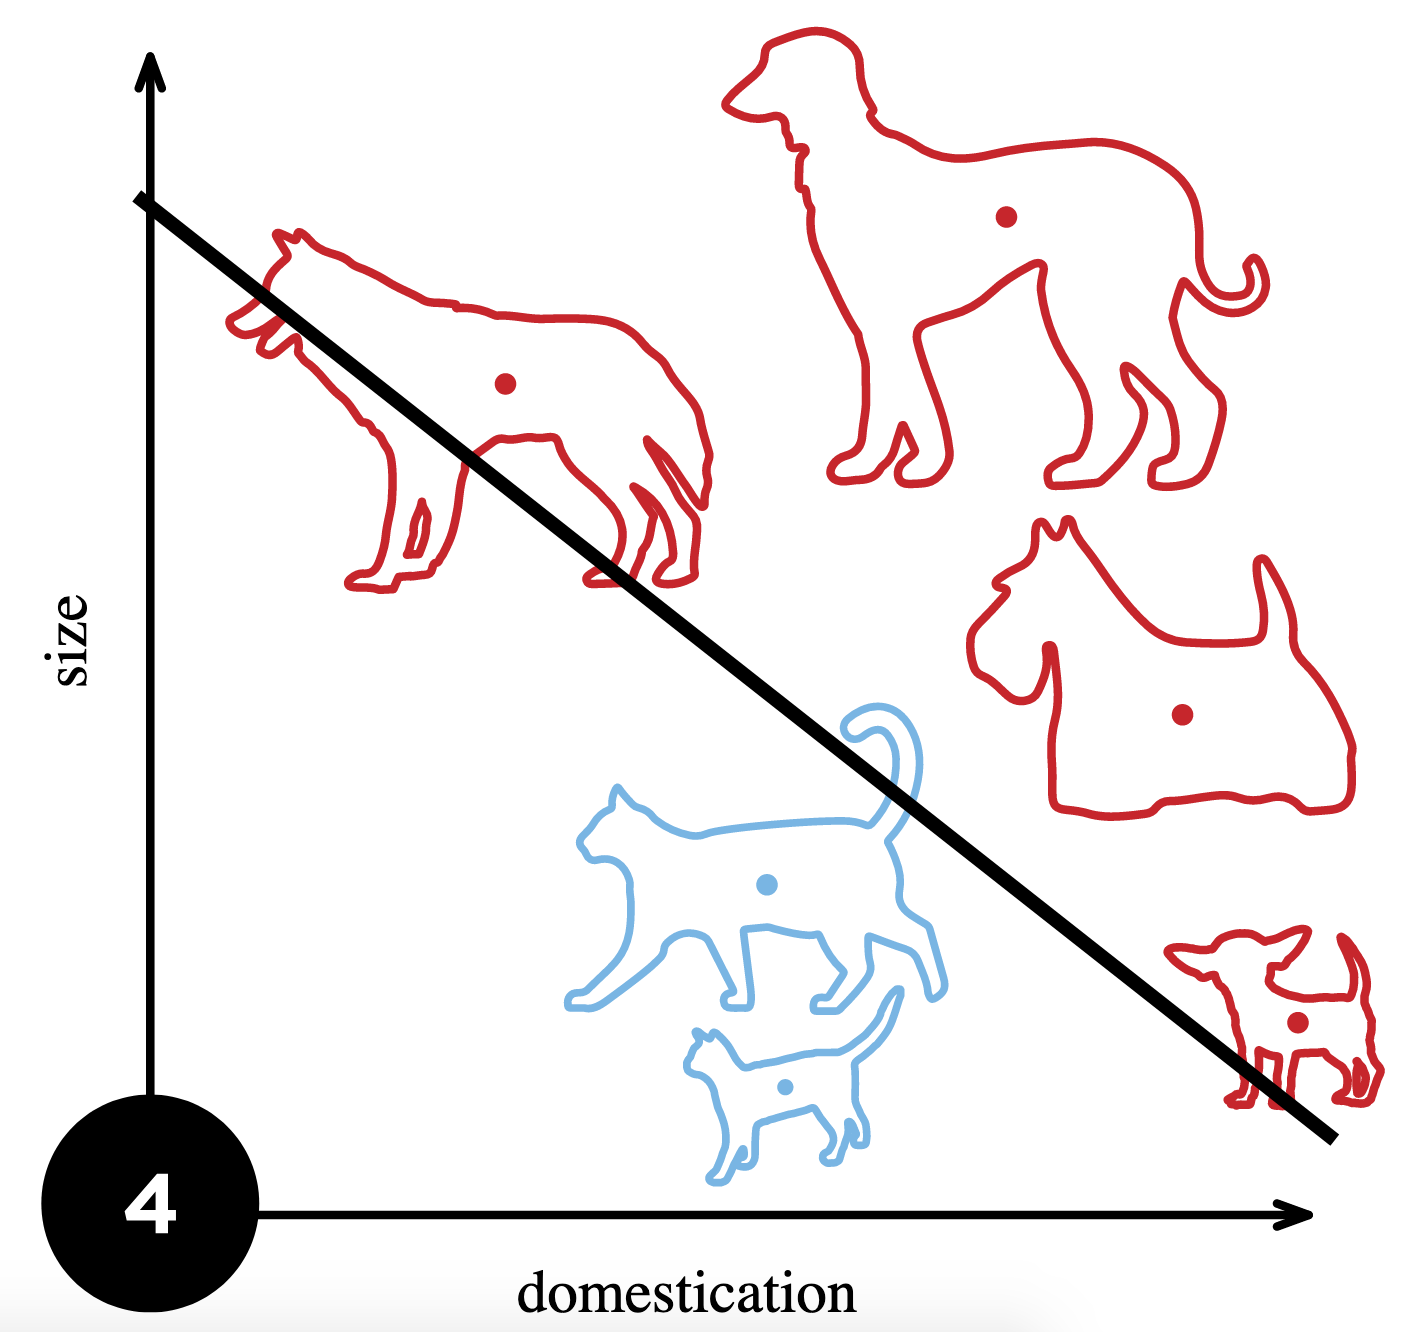
\includegraphics[width=0.7\textwidth]{figures/perceptron}
    \caption{An algorithm that learns to classify between dogs and cats is
      actually just learning where to put a line in the size $\times$
      domestication plane. \label{fig:perceptrong} }
  \end{figure}
\end{frame}

\begin{frame}
  \frametitle{Sensing: Gaussian Mixture Model}
 \begin{figure}[ht]
   \centering
   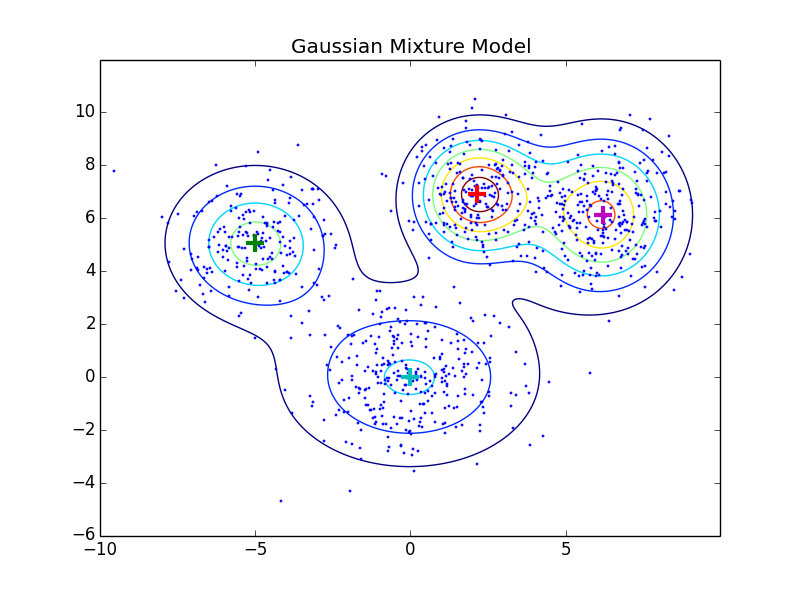
\includegraphics[width=0.7\textwidth]{figures/gmm}
   \caption{Example of a model that allows us to comparess lots of datapoints
     down to just a few representatives. \label{fig:gmm} }
 \end{figure}
\end{frame}

\begin{frame}
  \frametitle{Sensing: Information Retrieval}
  \begin{figure}[ht]
    \centering
    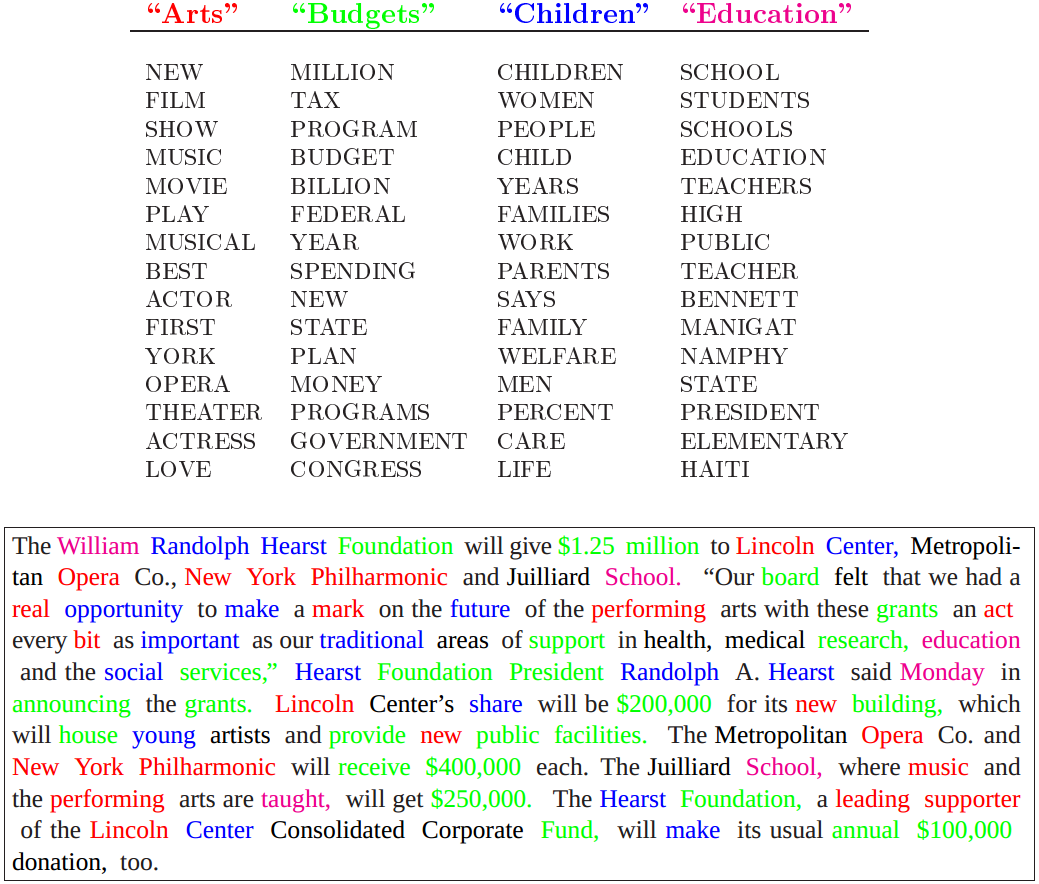
\includegraphics[width=0.7\textwidth]{figures/topics}
    \caption{This geometric view can inform many practical applications (like
      information retrieval, displayed here).\label{fig:topics} }
  \end{figure}
\end{frame}

\begin{frame}
  \frametitle{Sensing: Traffic in Jakarta}
  \begin{figure}[ht]
    \centering
    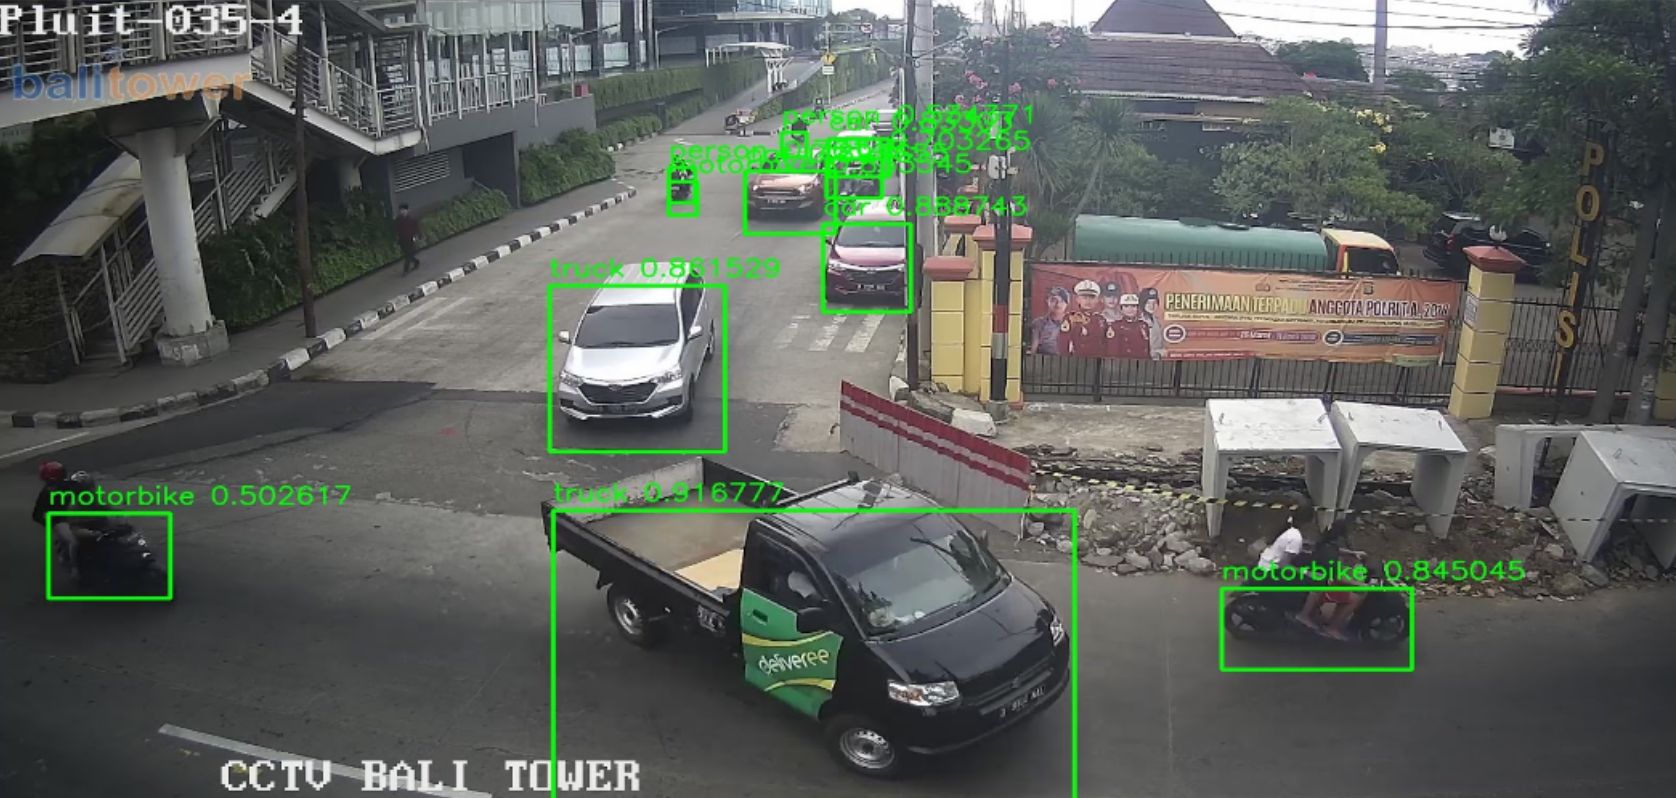
\includegraphics[width=0.9\paperwidth]{figures/jakarta_traffic}
    \caption{Automatically parsing traffic camera images can help with traffic
      management. \citep{caldeira2018improving} \label{fig:jakarta} }
  \end{figure}
\end{frame}

\begin{frame}
  \frametitle{Sensing: Conservation through Land Use Maps}
  \begin{figure}[ht]
    \centering
    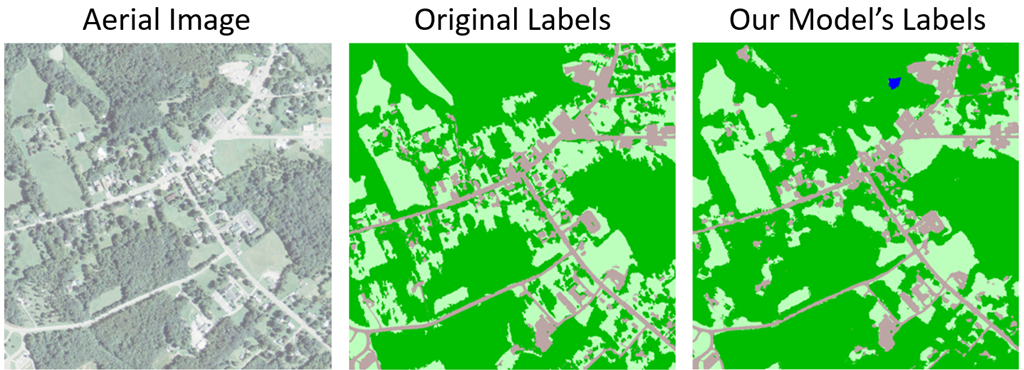
\includegraphics[width=0.7\paperwidth]{figures/landcover}
    \caption{Automatically generated land use maps let conservation
      organizations manage ecosystems. \label{fig:landcover} }
  \end{figure}
\end{frame}

\begin{frame}
  \frametitle{There is no magic in ML}
  \begin{figure}[ht]
    \centering
    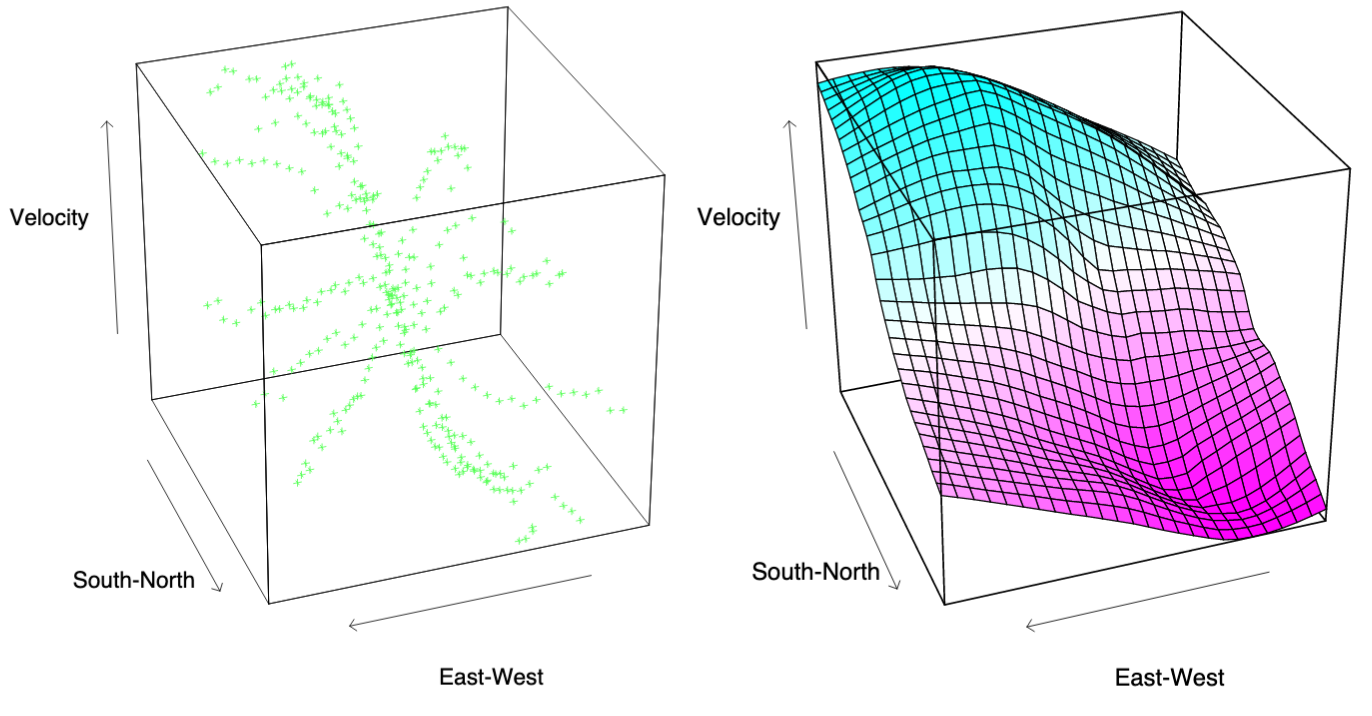
\includegraphics[options]{figures/galaxy}
    \caption{An example of regression, where we try to predict one value based
      on a bunch of related features. \label{fig:astronomy} }
  \end{figure}
\end{frame}

\begin{frame}
  \frametitle{Acting: Movie Recommendations}
  \begin{figure}[ht]
    \centering
    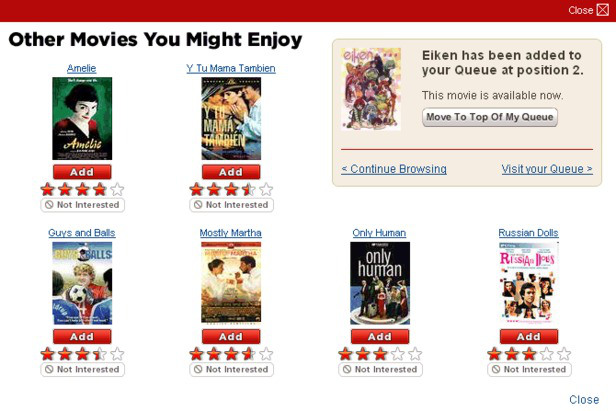
\includegraphics[width=0.7\textwidth]{figures/netflix_abstraction}
    \caption{Machine learning guides our decisions about which movies to watch.}
  \end{figure}
\end{frame}

\begin{frame}
  \frametitle{Acting: Movie Recommendations}
  \begin{figure}[ht]
    \centering
    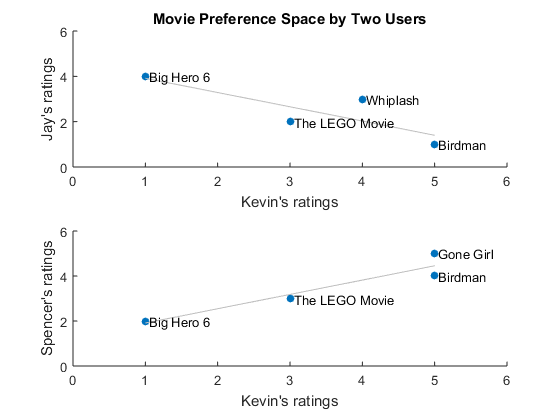
\includegraphics[width=0.7\textwidth]{figures/netflix_regression}
    \caption{Machine learning guides our decisions about which movies to watch.}
  \end{figure}
\end{frame}

\begin{frame}
  \frametitle{Acting: Lead Inspection}
  \begin{figure}[ht]
    \centering
    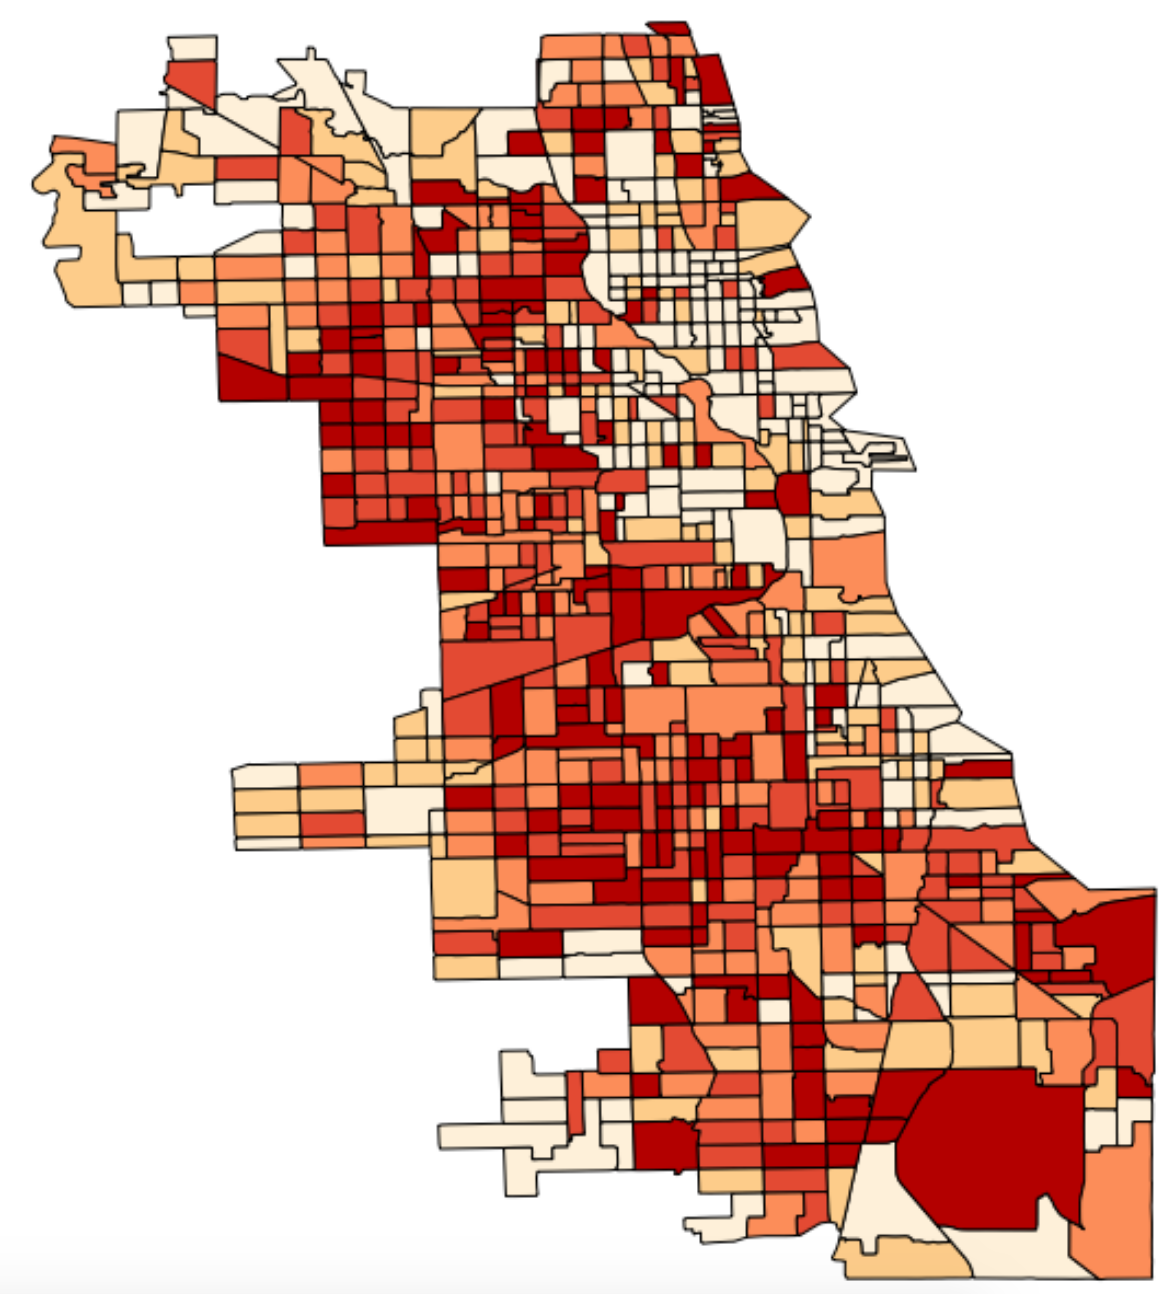
\includegraphics[width=0.7\textwidth]{figures/lead_inspection}
    \caption{Predictions about what homes will have lead can help guide inspections \citep{potash2015predictive}. \label{fig:potash_predictive} }
  \end{figure}
\end{frame}

\begin{frame}
  \frametitle{Acting: Agricultural Disease Detection}
  \begin{figure}[ht]
    \centering
    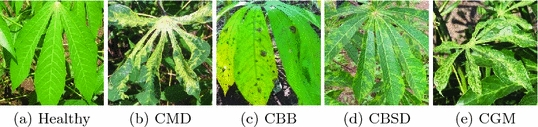
\includegraphics[options]{figures/cassava}
    \caption{A leaf classification system can help agricultural extension
      workers decide which areas need which treatments. \label{fig:cassava} }
  \end{figure}

\end{frame}

\section{ML Challenges}
\label{sec:label}

\begin{frame}
  \frametitle{Challenges}

  I've shown you a few of the success stories... but in practice many things
  remain challenges, especially in humanitarian applications.

  \begin{itemize}
  \item Data Collection
  \item Generalization
  \item Incompleteness
  \end{itemize} 
\end{frame}

\subsection{Data Collection}
\label{subsec:label}

\begin{frame}
  \frametitle{Training Examples}
  \begin{itemize}
  \item Most successful systems have automatically generated labels
  \item These can be hard (or expensive) to acquire in humanitarian applications
  \end{itemize} 
\end{frame}

\begin{frame}
  \frametitle{Training Examples}
  \begin{itemize}
  \item Most successful systems have automatically generated labels
  \item These can be hard (or expensive) to acquire in humanitarian applications
  \end{itemize} 
  \begin{figure}[ht]
    \centering
    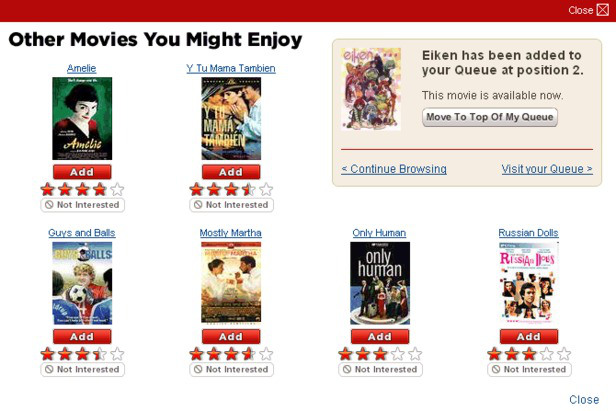
\includegraphics[width=0.7\textwidth]{figures/netflix_abstraction}
    \caption{Netflix obtains labels whenever you rate a movie. \label{fig:label} }
  \end{figure}
\end{frame}

\begin{frame}
  \frametitle{Training Examples}
  \frametitle{Training Examples}
  \begin{itemize}
  \item Most successful systems have automatically generated labels
  \item These can be hard (or expensive) to acquire in humanitarian applications
  \end{itemize} 
  \begin{figure}[ht]
    \centering
    \includegraphics[width=0.7\textwidth]{figures/flyinglabs.png
    \caption{Google learns from which search result you click
      on. \label{fig:label} }
  \end{figure}
\end{frame}

\begin{frame}
  \frametitle{Some Issues: Not enough labels}
  \begin{figure}[ht]
    \centering
    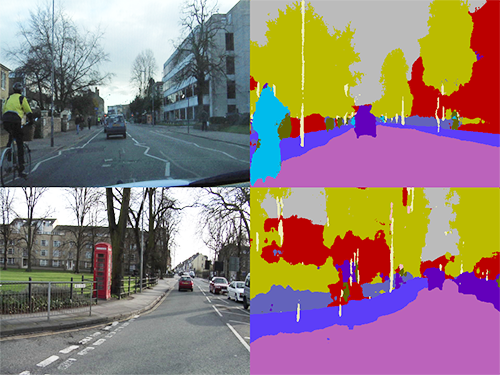
\includegraphics[width=0.7\textwidth]{figures/segmentation_labels}
    \caption{It's often much easier to obtain unlabeled data, compared to
      labeled data. \label{fig:label} }
  \end{figure}

\end{frame}

\begin{frame}
  \frametitle{Some Issues: Lack of representation}
\begin{figure}[ht]
  \centering
  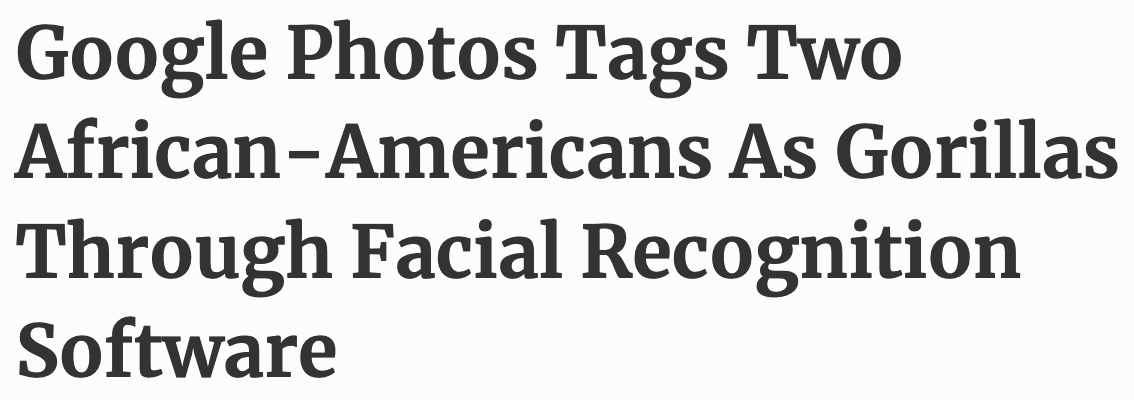
\includegraphics[width=0.7\textwidth]{figures/unrepresentative}
  \caption{If the model is not given representative labels, it will fail to
    perform well. \label{fig:label} }
\end{figure}
\end{frame}

\begin{frame}
  \frametitle{Some Issues}
\begin{figure}[ht]
  \centering
  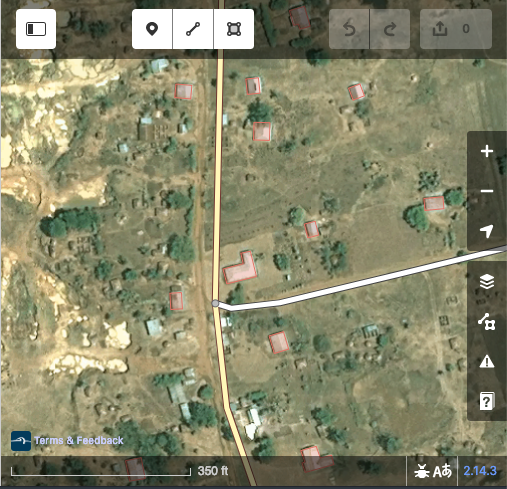
\includegraphics[width=0.7\textwidth]{figures/labeling}}
  \caption{In the real-world, labels may be partial or noisy, and models need to
    learn to be robust to (and ideally, continue to learn from) this.}
  \label{fig:label} }
\end{figure}
\end{frame}

\begin{frame}
  \frametitle{Solutions: Smarter labeling}
\begin{figure}[ht]
  \centering
  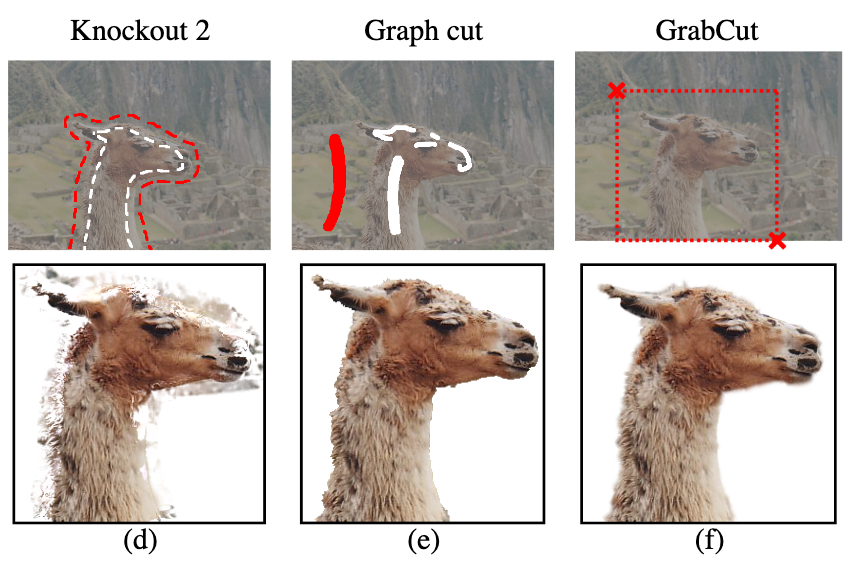
\includegraphics[width=0.7\textwidth]{figures/grabcut}
  \caption{There is work on building better interfaces for labeling data, for
    use in downstream algorithms. \label{fig:label} }
\end{figure}
\end{frame}

\begin{frame}
  \frametitle{Solutions: Active Learning}
  \begin{figure}[ht]
    \centering
    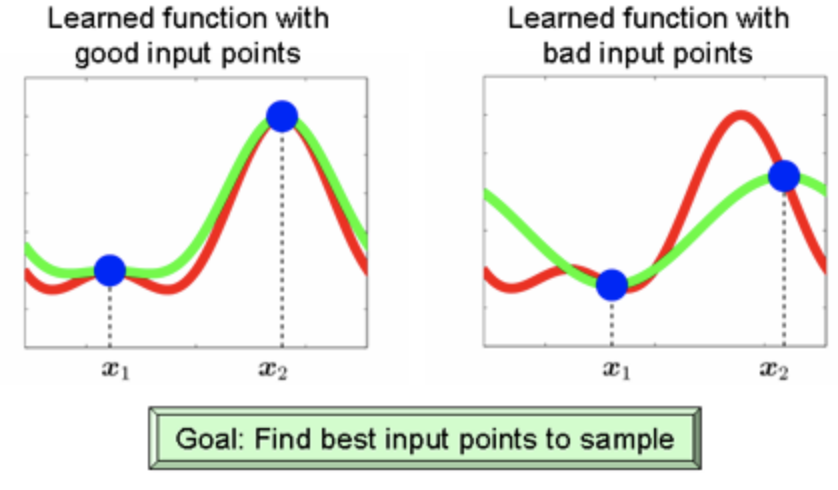
\includegraphics[options]{figures/active_learning}
    \caption{Rather than labeling datapoints at random, you could find a smart
      way of sorting through them. \label{fig:label} }
  \end{figure}
\end{frame}

\begin{frame}
  \frametitle{Solutions: Leverage Existing Infrastructure}
  \begin{figure}[ht]
    \centering
    \includegraphics[options]{figures/hotosm}
    \caption{It is foolish to attempt to fully automate systems with strong
      existing volunteer infrastructure. \label{fig:label} }
  \end{figure}
\end{frame}

\subsection{Generalization}
\label{subsec:label}

\begin{frame}
  \frametitle{Heterogeneity}
  Picture with just functions
\end{frame}

\begin{frame}
  \frametitle{Heterogeneity}
  Real world manifestations of this scenario: across place

  Self driving cars: Snow
\end{frame}

\begin{frame}
  \frametitle{Heterogeneity}
  Real world manifestations of this scenario: across time

  Nonstationarity: Airline waiting times have changed over time
\end{frame}

\begin{frame}
  \frametitle{Heterogeneity}
  Real world manifestations of this scenario

  Remote sensing: INRIA
\end{frame}

\begin{frame}
  \frametitle{Heterogeneity}
  Real world manifestations of this scenario

  Open Aerial Maps
\end{frame}

\begin{frame}[]
  \frametitle{Solutions}
  Traditionally: Just collect more data
\end{frame}

\begin{frame}[]
  \frametitle{Solutions}
  Metalearning: Train models that are more robust from the start?
\end{frame}

\begin{frame}[]
  \frametitle{Solutions}
  Active and reinforcement learning
\end{frame}

\begin{frame}[]
  \frametitle{Solutions}
  Causality: Gravity works on the moon
\end{frame}

\subsection{Incompleteness}
\label{subsec:label}

\begin{frame}
  \frametitle{Overview}
  Hard to specify everything into an objective function
  Need some assurance that we won't encounter unintended consequences
\end{frame}

\begin{frame}
  \frametitle{Models aren't perfect}
 Cemetaries and cars 
\end{frame}

\begin{frame}
  \frametitle{Examples}
  Examples from the Kim paper
\end{frame}

\begin{frame}
  \frametitle{Examples}
  Examples from the Kim paper
\end{frame}

\begin{frame}
  \frametitle{Remote Sensing}
  Would like results to be easily validatable / incorporatable.
\end{frame}

\begin{frame}
  \frametitle{Interpretability}
  Description of concepts
\end{frame}

\begin{frame}
  \frametitle{Interpretability}
  Examples of model distillation
\end{frame}

\section{Contextual Challenges}
\label{sec:label}

\begin{frame}
  \frametitle{Packaged Interventions}
  We like to think that technology alone will make our lives easier
  We often overlook the importance of context and intent.
\end{frame}

\begin{frame}
  \frametitle{Packaged Interventions}
  One laptop per child: Much easier to give people laptops than to ensure that
  teachers are well trained and showing up to the classroom.
\end{frame}

\begin{frame}]
  \frametitle{Packaged Interventions}
  In reality, solutions are very context dependent.
  Example with fishing villages in India and Uganda.
\end{frame}

\begin{frame}
  \frametitle{Theory of Amplification}
  Groups that have problems with existing infrastructure are unlikely to become
  better just because you give them
\end{frame}

\section{The Road Ahead}
\label{sec:label}

\begin{frame}
  \frametitle{Cognitive Amplification}
  Connect augmentation and tech amplification.
  The greatest promise of ML is in augmenting our cognition: Can we sensing
  better, and guide our decision making, in the most meaningful way possibl.
  Empower those who are already doing good work, via AI.
\end{frame}

\begin{frame}
  \frametitle{As we may Think}
  Let's take the long view, and keep things in perspective
\end{frame}

\begin{frame}
  \frametitle{Conclusion}
  Thank you for listening. I think you are all doing excellent work, and reach
  out if you have ideas about how we may be able to amplify your work.
\end{frame}

\bibliographystyle{plain}
\bibliography{refs}

\end{document}
